\subsection{ControlNet}
In 2023, Lvmin Zhang, Anyi Rao and Maneesh Agrawala from the Stanford University introduced a method for adding conditional control to text-to-image diffusion models~\cite{zhang2023addingconditionalcontroltexttoimage}. They dubbed this neural network architecture ``ControlNet''. ControlNet adds conditional control to pretrained neural network blocks by incorporating a secondary, trainable network. The process involves freezing the parameters of the original model blocks (e.g., ResNet or transformer blocks) and creating a trainable copy that receives external conditioning vectors. We first describe the basic architecture of ControlNet and a more concrete example of how Zhang et al.\ applied it to Stable Diffusion, followed by the training of ControlNet. Lastly, we discuss some things to be noted for inference like classifier-free guidance resolution weighting and how to combine multiple conditions. 

\subsubsection{Architecture}
ControlNet's functioning can be described by looking at what happends to the individual network blocks. Let $\mathcal{F}(\cdot; \Theta)$ be a neural block with parameters $\Theta$ that transforms an input feature map $x$ into an output feature map $y$:
\[
y = F(x; \Theta).
\]
\noindent
To integrate ControlNet, the parameters $\Theta$ of the original block are frozen/locked, and the block is cloned into a trainable copy with new parameters $\Theta_c$, as seen in Figure~\ref{fig:control_net:network_blocks}. The copy also takes an external conditioning vector $c$ as input. This configuration preserves the original model's robust capabilities while allowing the trainable copy to handle the input conditions.
\begin{figure}
    \centering
    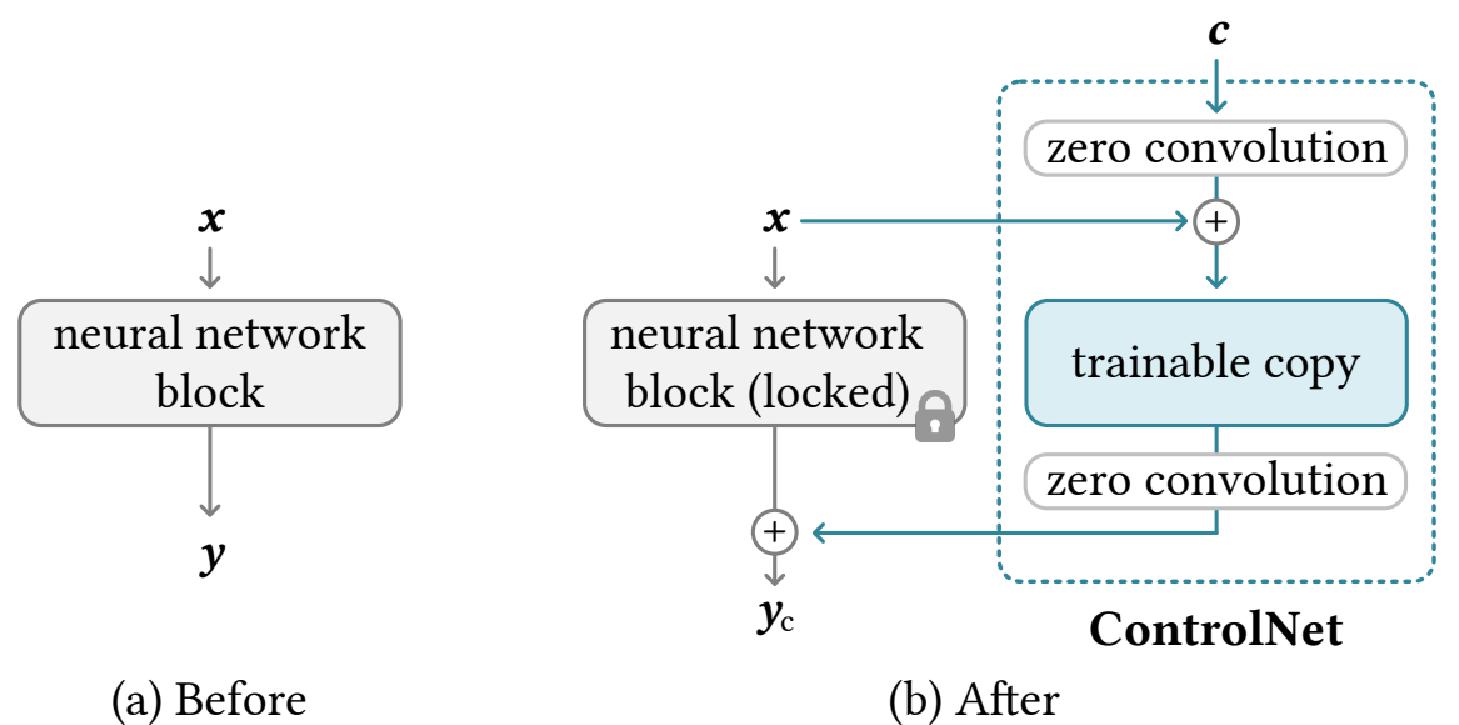
\includegraphics[width=0.7\textwidth]{assets/control_net_network_blocks.pdf}
    \caption{A visualization from Zhang et al.~\cite{zhang2023addingconditionalcontroltexttoimage} of a neural block that takes a feature map $x$ as input and outputs another feature map $y$, as shown in (a). The ControlNet is added by locking the original block and create a trainable copy. They are connected using zero convolution layers with both weight and bias initialized to zero. The conditioning vector $c$ is added to the network, as shown in (b)}
    \label{fig:control_net:network_blocks}
\end{figure}
The trainable copy is connected to the original block via zero convolution layers, denoted as $Z(\cdot; \cdot)$. These are $1 \times 1$ convolutions initialized with zero weights and biases, ensuring no interference at the start of training. ControlNet uses two such zero convolutions, with parameters $\Theta_{z1}$ and $\Theta_{z2}$. The complete computation in ControlNet is defined as:
\[
y_c = \mathcal{F}(x; \Theta) + \mathcal{Z}(\mathcal{F}(x + \mathcal{Z}(c; \Theta_{z1}); \Theta_c); \Theta_{z2}),
\]
where $y_c$ is the output of the ControlNet block. Initially, due to zero-initialization of the convolutions, $\mathcal{Z}(\cdot; \cdot)$ evaluates to zero, simplifying the equation to:
\[
y_c = y.
\]
This ensures that noise does not affect the neural network's hidden states during early training. As $\mathcal{Z}(c; \Theta_{z1}) = 0$, the trainable copy operates with the original input $x$, preserving the pre-trained model's functionality while serving as a reliable backbone for further learning. Zero convolutions effectively shield the backbone from random noise in the initial gradients, supporting stable training from the start. This method allows ControlNet to utilize the strengths of large-scale pretrained models effectively, applying them to diverse conditions without the risk of catastrophic forgetting or degradation of the pretrained model's performance. 

\subsubsection{Adding ControlNet to Stable Diffusion}
We demonstrate Zhang et al.'s integration of ControlNet with a large pretrained diffusion model using Stable Diffusion~\cite{rombach2022stablediffusion}. Stable Diffusion is structured as a U-Net~\cite{ronneberger2015unetconvolutionalnetworksbiomedical} comprising an encoder, a middle block, and a skip-connected decoder. The encoder and decoder each consist of 12 blocks, and the entire model has 25 blocks, including the middle block. Of these 25 blocks, 8 are down-sampling or up-sampling convolution layers, and the remaining 17 are main blocks, each containing 4 ResNet layers and 2 Vision Transformers (ViTs). Each ViT includes cross-attention and self-attention mechanisms. For example, in Figure~\ref{fig:control_net:sd_architecture}a, the ``SD Encoder Block A'' comprises 4 ResNet layers and 2 ViTs, and the ``$\times$3'' notation indicates this block repeats three times. Text prompts are encoded using the CLIP text encoder~\cite{radford2021learningtransferablevisualmodels}, and diffusion timesteps are encoded with a positional time encoder.
\begin{figure}
    \centering
    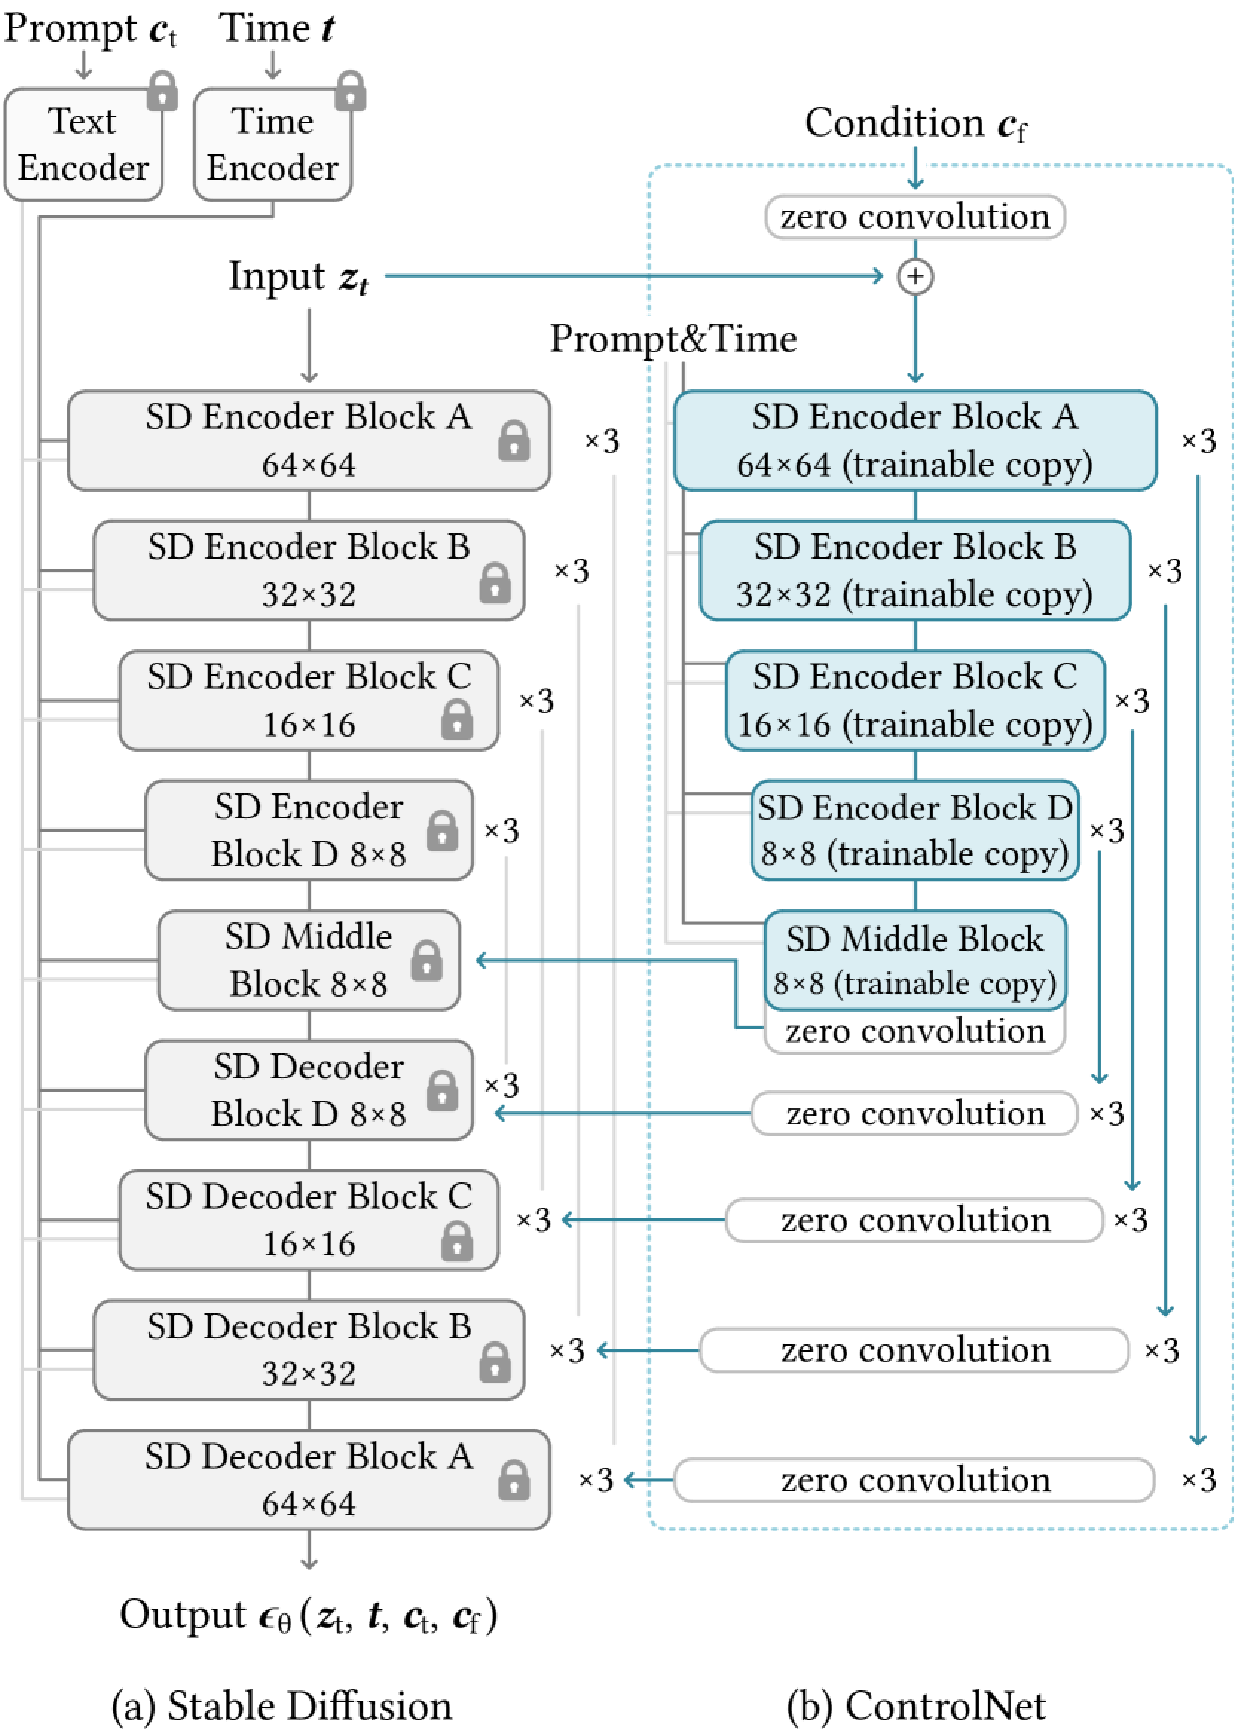
\includegraphics[width=0.7\textwidth]{assets/control_net_sd_architecture.pdf}
    \caption{A simplified description used in ``Adding Conditional Control to Text-To-Image Diffusion Models''~\cite{zhang2023addingconditionalcontroltexttoimage} to explain ControlNet's architecture in conjunction with Stable Diffusion. On the left side, in gray, we can see (a) Stable Diffusion's U-Net architecture, which parameters are frozen for the training of ControlNet. The (b) ControlNet, in blue, can be seen on the right. Just like Stable Diffusion it receives the prompt $c_t$, the time $t$ and noise $z_t$ as inputs, the only difference being, that it also allows for the task-specific conditions feature vector $c_f$ to be used.}
    \label{fig:control_net:sd_architecture}
\end{figure}
ControlNet is applied to each encoder level of the U-Net, as seen in Figure~\ref{fig:control_net:sd_architecture}b. Specifically, ControlNet creates trainable copies of the 12 encoding blocks and 1 middle block from Stable Diffusion. The 12 encoding blocks are distributed across 4 resolutions (64~$\times$~64,~32~$\times$~32,~16~$\times$~16,~8~$\times$~8), with each resolution level replicated three times. The outputs are added to the 12 skip-connections and 1 middle block of the U-Net. Given that Stable Diffusion follows a typical U-Net architecture, this ControlNet configuration can be extended to other models. ControlNet is computationally efficient since the frozen parameters do not require gradient computation during fine-tuning, reducing the load on the locked encoder. This approach accelerates training and conserves GPU memory. Zhang et al.\ report that, on a single NVIDIA A100 PCIE 40GB, optimizing Stable Diffusion with ControlNet uses about 23\% more GPU memory and 34\% more time per training iteration than without ControlNet.

Image diffusion models learn by progressively denoising and generating samples within the training domain, which can occur in pixel space or latent space. In Subsection~\ref{heading:subsection:stable_diffusion}, we explained the inner workings of Stable Diffusion and its operation in the latent space. It preprocesses 512 $\times$ 512 images into 64 $\times$ 64 latent representations. To add ControlNet, input conditioning images (e.g., edges, poses, depth) of size 512 $\times$ 512 are converted to a matching 64 $\times$ 64 feature space using a small encoder network $E(\cdot)$ composed of four convolution layers with 4 $\times$ 4 kernels and 2 $\times$ 2 strides, activated by ReLU and using channels [16, 32, 64, 128]. These layers are initialized with Gaussian weights and trained alongside the full model. The resulting feature space conditioning vector $c_f$ is computed as:
\[
c_f = E(c_i),
\]
where $c_i$ is the input condition, and $c_f$ is passed into the ControlNet.

\subsubsection{Training}
In image diffusion models, noise is progressively added to an initial image $z_0$, resulting in a noisy image $z_t$ after $t$ steps. Given conditions such as the timestep $t$, text prompts $c_t$, and a task-specific condition $c_f$, the network $\epsilon_\theta$ learns to predict the noise in $z_t$ using the objective:
\[
\mathcal{L} = \mathbb{E}_{z_0, t, c_t, c_f, \epsilon \sim \mathcal{N}(0, 1)} \left[ \| \epsilon - \epsilon_\theta(z_t, t, c_t, c_f) \|_2^2 \right],
\]
where $\mathcal{L}$ represents the overall learning objective of the diffusion model, and it is directly employed for fine-tuning with ControlNet. During training, Zhang et al.~\cite{zhang2023addingconditionalcontroltexttoimage} randomly replace 50\% of the text prompts $c_t$ with empty strings, which enhances ControlNet's ability to directly understand semantic information from conditioning images (e.g., edges, poses, depth) as a substitute for text prompts. Because zero convolution layers prevent noise addition, the model consistently predicts high-quality images. Furthermore, Zhang et al.\ observerd that ControlNet suddenly learns to follow the input condition from one optimization step to another, usually within 10.000 steps. They dubbed this the ``sudden convergence phenomenon''. It can be observed in Figure~\ref{fig:control_net:training_steps}, where different optimization steps and their corresponding outputs are shown.
\begin{figure}[h!]
    \centering
    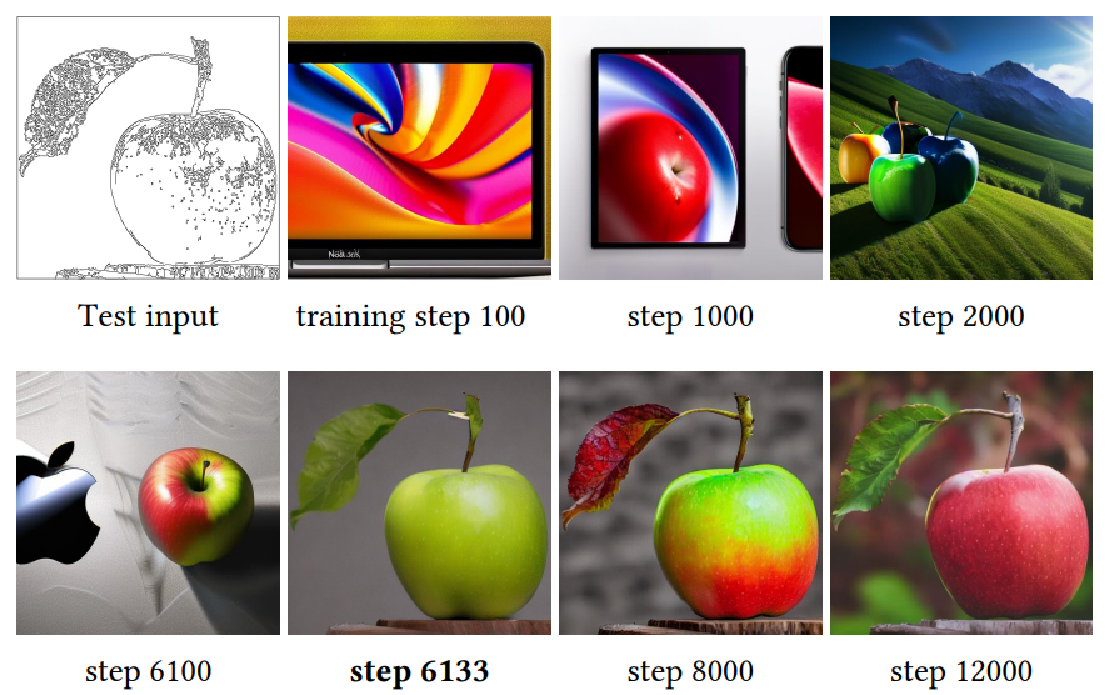
\includegraphics[width=0.7\textwidth]{assets/control_net_training_steps.pdf}
    \caption{The demonstration of the ``sudden convergence phenomenon'' used by Zhang et al.~\cite{zhang2023addingconditionalcontroltexttoimage}. The model abruptly learns to follow the input condition at a specific step in the training process (in this case step 6133 marked in bold).}
    \label{fig:control_net:training_steps}
\end{figure}